\section{Carte de puissance}
La carte de puissance est une carte permettant de faire l'interface entre le FPGA et les moteurs. En effet un FPGA ne peux délivrer la puissance necessaire à alimenter les moteurs.
Cette carte va s'articuler autour de deux composants principaux, deux ponts en H (LMD18200 de National Semiconductor), ces deux ponts permettront d'y connecter deux moteurs à
courant continu entre 12V et 55V qui consomment jusqu'à 3A.

Ces composants ne necessitent que l'ajout de quelque capacités de découplages pour fonctionner correctement. La carte est donc très simple et n'a consisté qu'en l'ajout de ces capacités et
de borniers afin de connecter l'alimentation principale, les PWM (une par moteur) et les moteurs.

\begin{figure}[h]
\centering
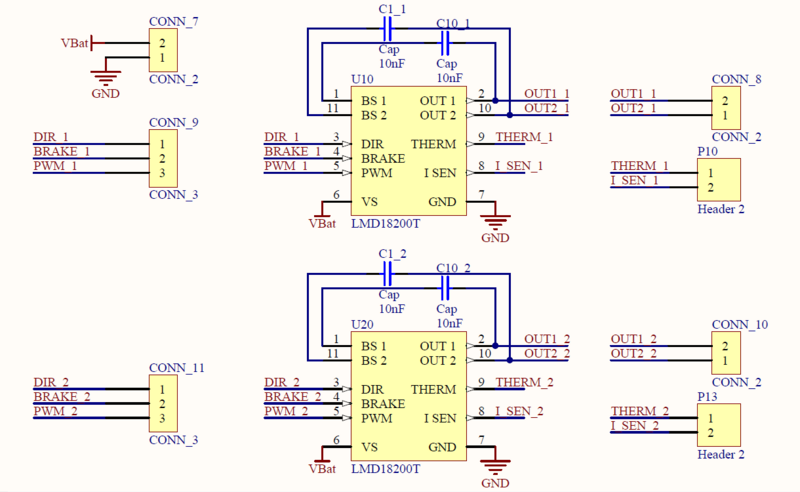
\includegraphics[width=17cm]{img/Schema_carte_puissance.PNG}
\caption{Schéma électrique de la carte de puissance}
\end{figure}
\pagebreak